 \section{Nary Relationship ODP}\begin{description}
\item [CLASSIFICATION:] Extension.

\item [MOTIVATION:] The biomedical domain is full of situations were relationships should hold between more than one element, but OWL only allows to express properties linking two individuals at a time. There can be a situation where a relationship and some properties of that relationship must be modelled; that can not be done in a direct manner with OWL. For example, a diagnosis has a result, a probability, and the person who has been diagnosed; A catalytic reaction has got a substrate, some products, catalytic constants and it is catalysed by an enzyme.

\item [AIM:] To express a relationship between more than one element. A Gene Ontology example can be found in the term GolgiToPlasmaMembrane CFTRproteinTransport, where there is a transport phenomenom which relates to three elements at the same time: the start (Golgi apparatus), the end (plasma membrane) and the transportee (CFTR protein). The transport relation can not be modelled in OWL pointing to the three elements, so this ODP must be applied.

\item [STRUCTURE:] See Figure \ref{odp:Nary_Relationship_abstract}.
\begin{figure}[]\centering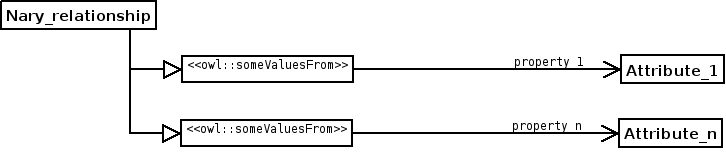
\includegraphics[width=\textwidth]{Catalogue/Nary_Relationship_abstract}\caption{\label{odp:Nary_Relationship_abstract} Abstract structure of the Nary Relationship ODP.}\end{figure}

\item [SAMPLE:] See Figure \ref{odp:Nary_Relationship_instance}.
\begin{figure}[]\centering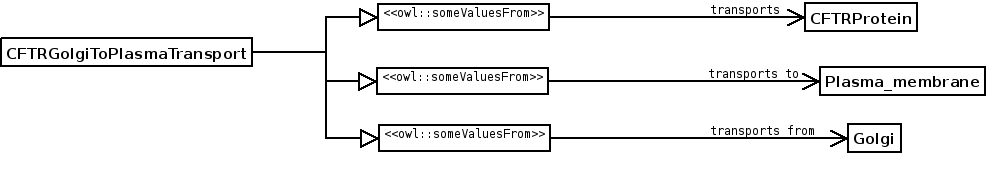
\includegraphics[width=\textwidth]{Catalogue/Nary_Relationship_instance}\caption{\label{odp:Nary_Relationship_instance} Sample structure of the Nary Relationship ODP.}\end{figure}

\item [ELEMENTS:] The original elements of the Nary Relationship are conserved in classes and a new class is reified to model the Nary Relationship, in this case a class called CFTRGolgiToPlasmaTransport. The relationships of each element to the reified class are created: TransportsFrom, TransportsTo and Transports.

\item [IMPLEMENTATION:] There is a Protege wizard available for easily creating N-ary Relationships.

\item [RESULT:] After the reification a N-ary relationship is stated in the ontology.

\item [SIDE EFFECTS:] The class that holds the Nary relationship must have a clear name, because the maintainer must know that the class is not a proper class, otherwise the ontology becomes confusing. Therefore naming consistency should be maintained if different Nary relationships are created.

\item [ADDITIONAL INFORMATION:] It could be argued that this is not really an ODP, as n-ary relationships in OWL do not exist, and, therefore, this would be a naming ODP instead of a semantic ODP, as the key of the pattern is how the class holding the alleged n-ary relationship is named.

\item [REFERENCES: ] ~\begin{itemize}
\item Robert Stevens, Mikel Egana Aranguren, Katy Wolnstencroft, Ulrike Sattler, Nick Drummond and Mathew Horridge. Using OWL to Model Biological Knowledge. International Journal of Human Computer Studies 2006, 65:7, 583-594.
\item \url{http://www.co-ode.org/resources/tutorials/bio/}
\item \url{http://www.w3.org/TR/swbp-n-aryRelations/}\end{itemize}
\item [URL: ] \url{http://www.gong.manchester.ac.uk/odp/owl/Extension_ODP/Nary_Relationship.owl} \end{description}